\chapter{字串\uppercase\expandafter{\romannumeral 1}}

\section{前言}
沒錯沒錯,今天要介紹的就是字串啦!

不知道大家知不知道字串和普通的序列差別是甚麼?其實字串本身就是一個序列,但通常在題目跟連續性有關的時候,我們才會稱它為字串題。

那就讓我們趕快進入此次的主題-字串吧!
\section{基礎名詞簡介}
\begin{enumerate}
\item 字元 (character):構成字串的單位。以下「字串 $A$ 的第 $i$ 個字元」簡寫為 $A_i$。
\item 字元集:所有可能的字元的集合。
\item 長度:一個字串的字元個數。以下將「字串 $A$ 的長度」簡寫為 $|A|$。
\item 子字串 (substring):一個字串的一段連續的字元所構成的字串稱作子字串。以下將
「字串 $A$ 的第 $[i, j]$ 個字串所構成的子字串」簡寫為 $A_{i...j}$。(注意本篇講義的字串為左閉右閉)
\item 前綴、後綴 (prefix,suffix):一個字串只取最前面一些字元所構成的子字串是前綴,只
取最後面的則是後綴。前綴可寫成 $A_{0...i}$、後綴可寫成 $A_{i...|A|-1}$。
\end{enumerate}

\section{字串匹配問題}
字串匹配是字串的經典老題。因為它太老,而不常出現在競賽中。不過字串匹配的眾多解法時常出現許多富有巧思的變化,用以解決較複雜的字串問題。現在讓我們來看看這個原始的問題吧!\\

\problem{字串匹配}{
	給你一個字串$T$,以及字串$P$。求$P$是否為$T$的其中一個子字串。
}

最基本的想法是枚舉起點,然後再一一往後配對,當匹配不上則將起點向右移動一格。這樣的複雜度會是$O(|P||T|)$。\\

\begin{C++}
bool matching(string t,string p){
    if(t.size() < p.size()) return false;
    for(int i = 0; i < t.size() - p.size() + 1; i++){
        bool found = true;
        for(int j = 0; j < p.size(); j++)
            if(t[j+i] != p[j]) found = false;
        if(found) return true;
    }
    return false;
}
\end{C++}

當然,這樣的複雜度對於每日處理龐大資料的電腦算是一場災難,所以我們需要更加快速的解決方案。

\subsection{雜湊 (Hash)}
在處理字串問題中所提到的hash通常都是指將字串轉換成為一個數字,這樣比較的時候就可以達到$O(1)$的比較時間了呢!做法就是將字串看長一個$p$進位制的數字,具體一點來說,假設雜湊函數為$h(A)$($A$是一個字串),則
\begin{math}
h(A) = A_0p^{|A|-1} + A_1p^{|A|-2} + ... + A_{|A|-1}
\end{math}
($|A|$為字串長度)。照理說,只要$p$比字元集大小還要大,那就可以將一個字串唯一的轉成一個數字了喔!好,接下來問題就是,要如何快速地找出一個字串中某個子字串的hash值呢?首先我們先預處理字串每個前綴的hash值,也就是找出$h(A_{1...|A|-1}), h(A_{1...|A|-2}),...,h(A_{1...1})$。根據定義,應該不難看出,$h(A_{1...i}) = h(A_{1...i-1})\times p + A_i$。因此,只需要花$O(|A|)$的時間就可以預處理完了。接著假設想要知道$A_{i...j}$這段子字串的湊湊值,一樣根據定義,這段的雜湊值就是$h(A_{1...j}) - h(A_{1...i})\times p^{j-i}$,而這個值可以$O(1)$算出(畢竟$p$的冪次也可以$O(|A|)$預處理然後$O(1)$知道。\\

這樣說是不是感覺非常簡單易懂呢?但或許大家也發現了,就是雜湊值會非常大,\inline{long long}也存不下嘛!而應對方式也非常簡單,就是在計算的時候模一個數字,就所有問題都解決了,因為上述的計算都可以在一個模數之下好好地做。但這樣也出現了新的問題,就是因為雜湊值模了一個數,有可能造成兩個不同的字串卻有相同的雜湊值,這就是碰撞(collision)囉。解決方式也很簡單,就是開很多hash,如果那麼多個hash值都顯示兩個字串相同,那我們或許就可以合理相信兩個字串真的一樣了呢。那到底要寫多少hash才合理呢?我聽說一般是要寫5個hash喔!\\

最後的問題就是$p$和模數的選取了,我不是很確定怎麼選才好,不過一般認為模數應該要夠大(要不然更容易碰撞),而且$p$和模數應該不互質的時候會有某些數不被用到,所以我會選把兩個都選成質數(或至少模數選質數)。\\

唉呀,講了這麼多,都還沒講到要怎麼用hash來匹配字串呢!\\

假設要在字串$A$中找到字串$B$,則我們一樣花$O(|A|)$的時間將$A$的每一個前綴的hash找出來,也順便算出$B$的hash值。接著我們可以知道,$A$中有$|A| - |B| + 1$個位子有可能找到$B$,因此,我們就可以在線性時間內去看每個可能符合條件的位子的hash值跟$B$一不一樣就做完囉!整體來說,用hash來做字串匹配的複雜度是$O(|A| + |B|)$。\\

Hash固然是字串匹配的好幫手,不過千萬不要覺得Hash只能拿來做字串匹配,有許多其他字串題也有它出場的機會!\\

以下附上我醜醜的 code。

\subsection{\inline{string::find}}
這個東西就是C++ STL裡面的函式,可以直接達到字串匹配的目的。直接給出範例程式囉!
\begin{C++}
#include<iostream>
#include<string>
using namespace std;
int main()
{
  string A = "ABCABCABC";
  string B = "CAB";
  cout << A.find(B) << endl;//在A中找出B第一個出現的位子
}
\end{C++}
感覺非常實用呢,是不是?但相信大家或許跟我一開始會有一樣的問題,就是它的複雜度到底是多少呢?我大概上網查了一下,C++沒有規定它的複雜度,但我實測起來感覺速度頗快,大家好好斟酌一下比賽的時候要不要用吧。

\section{古斯菲爾德演算法}

這個字串匹配的演算法由 Dan Gusfield 提出,又稱作 Z-algorithm。這個演算法能夠實現,主要是建立在「對於一個字串$s$,能夠在線性時間內計算其對應的Z-陣列」 這個基礎上。\\

\subsection{Z-陣列}

\textbf{Z-陣列}是一個與字串長度相同的陣列,每個元素$Z[k]$代表的是以位置$k$為始的最長子字串長度,使得這個子字串也是整個字串的前綴。\\

以字串\inline{ACBACDACBACBACDA} 為例,依此建構出的Z-陣列就如以下所示:\\

\begin{center}
\begin{tikzpicture} [nodes in empty cells,
      nodes={minimum width=0.7cm, minimum height=0.7cm},
      row sep=-\pgflinewidth, column sep=-\pgflinewidth]
      border/.style={draw}
    
      \matrix(vector)[matrix of nodes,
          row 1/.style={nodes={draw=none, minimum width=0.3cm}},
          nodes={draw}]
      {
          \scriptsize{0} & \scriptsize{1} & \scriptsize{2} & \scriptsize{3} & \scriptsize{4} & \scriptsize{5} & \scriptsize{6} & \scriptsize{7} & \scriptsize{8} & \scriptsize{9} & \scriptsize{10} & \scriptsize{11} & \scriptsize{12} & \scriptsize{13} & \scriptsize{14} & \scriptsize{15}\\
          \inline{\inline{A}} & \inline{C} & \inline{B} & \inline{A} & \inline{C} & \inline{D} & \inline{A} & \inline{C} & \inline{B} & \inline{A} & \inline{C} & \inline{B} & \inline{A} & \inline{C} & \inline{D} & \inline{A}\\
          $16$ & $0$ & $0$ & $2$ & $0$ & $0$ & $5$ & $0$ & $0$ & $7$ & $0$ & $0$ & $2$ & $0$ & $0$ & $1$\\
      };
\end{tikzpicture}
\end{center}

其中$Z[6]=5$,因為以$s[6]$開頭的子字串\inline{ACBACB}剛好是整個字串的一個前綴。\\

\subsection{如何計算Z-陣列}

計算Z-陣列的方法正是Gusfield's Algorithm的精神所在。為了有效率的完成Z-陣列的建構,這個演算法會維護一個區間$s[x...y]$,使得這個區間是一個原字串的前綴,而且$y$要盡量越大越好。\\

維護這個區間的目的是:當你要計算一個未知的$Z[i]$時,能夠確保可以利用先前儲存的值快速計算。如果將要計算$Z[i]$的$i$在$s[x...y]$的區間之外,我們就沒有儲存到任何有關$Z[i]$的資訊,只能從頭計算;但是如果這個$i$在這個區間內,就可以很快知道$Z[i]$至少有$\min(Z[i-x], y-i+1)$,所以從這個值開始暴力搜就行了。\\

詳細作法如下:
\begin{enumerate}
\item 如果 $i>y$,代表還沒有已知的、與前綴相同的子字串包含$i$,這時候重新暴力比對$s[0...$ 與 $s[i...$,並更新$x, y, Z[i]$。
\item 如果 $i\leq y$我們知道$s[0...y-x]$ 與 $s[x...y]$ 相等,因此 $i$ 的位置在 $s[x...y]$ 的地位就類似 $i-x$ 在 $s[0...y-x]$ 的地位。因此我們可以用 $Z[i-x]$ 來推算 $Z[i]$。
\item 如果 $Z[i-x] < y-i+1$,已經確定 $Z[i]$ 不能再多了,所以 $Z[i]$ 就是 $Z[i-x]$。
\item 如果 $Z[i-x] \geq y-i+1$,那麼 $Z[i]$ 只能確定不小於 $y-i+1$,所以一樣要暴力比對$s[y...$ 與 $s[y-x...$,並更新$x, y, Z[i]$。
\end{enumerate}

\begin{C++}
vector<int> Z(string &s){
    vector<int> Z(s.size());
    int x = 0, y = 0;
    for(int i = 0; i < s.size(); i++){
        Z[i] = max(0, min(y-i+1, Z[i-x]));
        while(i+Z[i] < s.size() && s[Z[i]] == s[i+Z[i]])
            x = i, y = i+Z[i], Z[i]++;
    }
    return Z;
}
\end{C++}

隨著越來越多的$Z[i]$被算出來,$y$值也會不斷的增加,每次暴力往後搜一格,$y$值就會增加或至少不變,所以需要暴力搜的個數不會超過$O(n)$。\\

也就是說,對於每個$i$,當\inline{while}迴圈的條件成立時頂多使$y$值不變一次,第二次開始$y$值一定會增加$1$。因為$y$值最多只有字串長度,所以時間複雜度$O(n)$。

\subsection{Z-陣列與字串匹配}

有了Z-陣列之後,那我們要怎麼進行字串匹配呢?這邊我們需要一些巧思,將$P$與$T$兩個字串用特殊字元接在一起,再做一次Z-陣列就行了。

\begin{center}
\begin{tikzpicture} [nodes in empty cells,
      nodes={minimum width=0.7cm, minimum height=0.7cm},
      row sep=-\pgflinewidth, column sep=-\pgflinewidth]
      border/.style={draw}
    
      \matrix(vector)[matrix of nodes,
          row 1/.style={nodes={draw=none, minimum width=0.3cm}},
          nodes={draw}]
      {
          \scriptsize{0} & \scriptsize{1} & \scriptsize{2} & \scriptsize{3} & \scriptsize{4} & \scriptsize{5} & \scriptsize{6} & \scriptsize{7} & \scriptsize{8} & \scriptsize{9} & \scriptsize{10} & \scriptsize{11} & \scriptsize{12} & \scriptsize{13} & \scriptsize{14} & \scriptsize{15}\\
          \inline{\inline{A}} & \inline{C} & \inline{B} & \inline{\#} & \inline{C} & \inline{D} & \inline{A} & \inline{C} & \inline{B} & \inline{A} & \inline{C} & \inline{B} & \inline{A} & \inline{C} & \inline{D} & \inline{A}\\
          $16$ & $0$ & $0$ & $0$ & $0$ & $0$ & $3$ & $0$ & $0$ & $3$ & $0$ & $0$ & $2$ & $0$ & $0$ & $1$\\
      };
\end{tikzpicture}
\end{center}

在這裡,Z-陣列中值恰好等於字串$P$長度的位置,就是找到了的$P$的一個匹配。

\section{克努斯-莫里斯-普拉特演算法}
除了 Gusfield's Algorithm 之外,還有一個類似的作法叫 KMP 算法,這個做法也是對於原字串建立一個陣列,再利用這個陣列的值進行字串匹配。

\subsection{失配函數}
想像一個情境:你嘗試用暴力法在 \inline{aaabaaaab} 找 \inline{aaaa} ,當你從第一個字元當開頭匹配到第四個字元時,你明明已經知道因為有個\inline{b}卡在那裡,導致前四個字元都不可能作為開頭。但是你還是必須把開頭對到第二個字元,再慢慢掃,對吧。\\

這時候你就需要一個東西,先對字串$P$計算好一個陣列,指引配對失敗時開頭位置要怎麼往後跳,就可以不必每次都只往後一格。

\subsection{次長共同前後綴}
失配函數事實上就是次長共同前後綴。我們定義 
\begin{displaymath}
Fail(i) = s[0...i] \mbox{\textit{的次長共同前後綴的長度}}
\end{displaymath}
這裡用次長不用最長的原因很簡單,因為最長共同前後綴就是$s[0...i]$本身,根本沒必要算。\\

那我們對於一個字串$P$,我們要怎麼建立失配函數陣列呢?\\

與Z-陣列的建構方式有些類似,對於每個 $i$,我們可以確定 $s[0...F[i-1]] = s[i-1-F[i-1]...i-1]$,因此可以假設 $q = F[i-1]$。如果$s[q]$ 與 $s[i]$相同,則 $F[i]$ 的值就等於 $q+1$。\\

如果這兩個字元不相同,我們可以試著縮小 $q$ 的值,來使$s[q]$ 與 $s[i]$相同。因為失配函數本身的性質,我們可以知道 ,$s[i-F[q-1]-1...i-1]$ 與 $s[0...F[q-1]]$ 是一樣的,所以可以將新的 $q$ 換成 $F[q-1]$,繼續比對 $s[q]$ 與 $s[i]$。\\

\begin{C++}
vector<int> build_failure(string &s){
    vector<int> fail = {0};
    for(int i = 1, q = 0; i < s.size(); i++){
        // q = fail[i-1];
        while(q && s[i] != s[q]) q = fail[q - 1];
        fail.push_back(q += (s[i] == s[q]));
    }
    return fail;
}
\end{C++}

\subsection{KMP與字串匹配}

相信有了失配函數之後,大家都很快就知道怎麼進行字串匹配了。我們先對欲尋找的字串$P$,建立它的失配函數陣列,然後用兩個變數 $i, j$ 在字串 $T$ 與 $P$ 上爬行。\\

如果 $T[i] = P[j]$ 表示配對正確,則繼續對 $T[i+1], P[j+1]$ 進行比對,直到字串完全匹配或失配;如果 $T[i] \neq P[j]$ 代表失配,將 $j$ 的值跳到失配函數 $(F[j-1])$ 的位置就行了! $j = |P|$ 時就代表 $P$ 字串已經被完全找到,達成字串匹配的目的。

\begin{C++}
void KMPSearch(string t, string p){
    vector<int> fail = build_failure(p);
    int i = 0; // index for t[]
    int j = 0; // index for p[]
    while (i < t.size()){
        if(p[j] == t[i]){ // 匹配
            j++, i++;
        }
        if(j == p.size()){ // 找到了!
            printf("Found pattern at index %d \n", i-j);
            j = fail[j-1];
        }
        else if(i < t.size() && p[j] != t[i]){ // 失配
            if(j != 0) j = fail[j-1];
            else i++;
        }
    }
}
\end{C++}
另一種比較短的寫法是
\begin{C++}
void KMPsearch(string t, string p) {
	vector<int> fail = build_failure(p);
	for(int i = 0, j = 0; i < t.size(); i++) {
		while(j && t[i] != p[j]) j = fail[j-1];
		if(t[i] == p[j]) ++j;
		if(j == p.size()) {
			printf("Found pattern at index %d \n", i-j);
			j = fail[j-1];
		}
	}
}
\end{C++}

\section{Trie}
首先考慮一個這樣的問題,你需要處理兩種操作:一、在資料結構中加入一個字串;二、給你一個字串,問你此字串是否曾經被插入該資料結構。大家或許會很直覺地認為直接開一個\inline{set},然後把字串全部丟進去就解決了!那這麼做的複雜度會是多少呢?假設目前有$N$個字串在\inline{set}中,而當前要查詢一個長度為$L$的字串是否在\inline{set}中,這樣複雜度就是$O(L\log N)$。有沒有可能有更好的複雜度呢?這時候就要派我們的Trie出場了呢!看看它的英文字首,就知道他絕對是跟樹有關了呢!它的的確確是一棵樹,它的每一顆節點都包含了字元集大小的那麼多個指標,舉例來說,若全部的字串都是由英文小寫字母所組成的話,那每顆節點都有26個指標。好,接下來就直接說要如何插入一個字串吧,直接來看例子比較直接:\\
下圖插入了"s", "so", "tp", "tip", "she", "x",灰色節點表示該節點是一個字串的結尾
\begin{center}

\iftrue
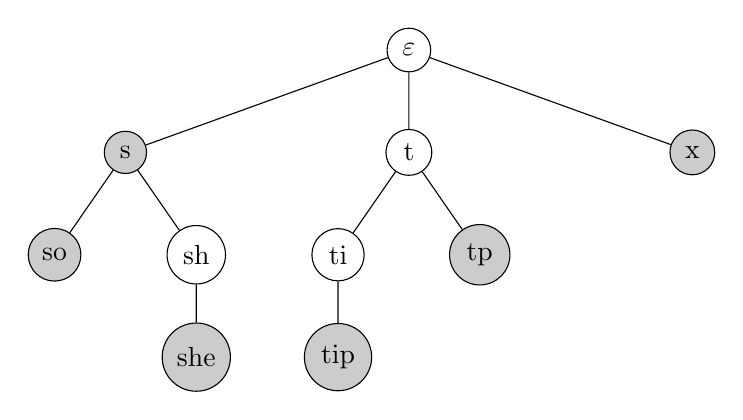
\begin{tikzpicture}[every node/.style={draw},
level 1/.style={sibling distance=36mm,circle,level distance=1.3cm},
level 2/.style={sibling distance=18mm,circle,level distance=1.3cm},
level 3/.style={sibling distance=12mm,circle,minimum width=7mm,minimum height=7mm}]
\node[circle]{$\varepsilon$}
	child { node[fill=black!20]{s} 
		child{ node[fill=black!20]{so} }
		child{ node{sh} 
			child{ node[fill=black!20]{she} }
		}
	}
	child { node{t} 
		child{ node{ti}
			child{ node[fill=black!20]{tip} }
		}
		child{ node[fill=black!20]{tp} }
	}
	child { node[fill=black!20]{x} }
;
\end{tikzpicture}
\fi
\end{center}
相信大家看完了上面的例子,都大概了解Trie的運作方式了。而它的時間複雜度大家應該也知道,就是插入和查詢都是$O(N)$,而空間複雜度就是$O($字元集大小$\times \sum L_i)$。其實gcc中的pbds也有一個能直接拿來用的Trie,詳情就參考pbds的講義吧!

在字元集越小的時候,Trie越容易派上用場,尤其是只有0跟1的時候,例如跟某些位元運算有關的題目常常得把Trie派出場。

\problem{最大區間XOR(經典問題)} {
給定一個序列,求最大的區間XOR值。
}
對序列做一次前綴可以發現問題變成找到兩個數字XOR起來最大,我們可以一個一個把前綴的二進位表示法丟進Trie裡面(最高位放在前面)並順便拿去Trie裡面查,能夠往相反的地方走就盡量往相反的地方走便能找到最大XOR值。

\begin{C++}
int ch[N*30][2], tot; // 0同時代表根節點和空節點:P
void ins(int x) {
	int now = 0;
	for(int c = 29; c >= 0; c--) {
		bool d = x>>c & 1;
		if(!ch[now][d])
			ch[now][d] = ++tot;
		now = ch[now][d];
	}
}
int qry(int x) {
	int now = 0, res = 0;
	for(int c = 29; c >= 0; c--) {
		bool d = x>>c & 1;
		if(ch[now][!d])
			now = ch[now][!d], res ^= 1<<c;
		else
			now = ch[now][d];	
	}
	return res;
}
\end{C++}
\section{習題}
排版跑掉了\ 郭死\\

\problem{Massacre at Camp Happy (TIOJ 1725)}{給定兩個長度相同的字串$A$、$B$,請你找出所有的$k$,使得將$A$的前$k$個字元移到尾端時會跟$B$只差一個字元,或回答不存在符合的$k$。($|A|,|B|\leq 10^6$)}
\problem{似曾相識 (TIOJ 1515)}{給定一字串$s$,請問在此字串中重複出現兩次以上的最長字串長度為何(若無則輸出0)?($|s|\leq 2\times 10^5$)(其實這題可以用一個較複雜的結構suffix array做完,但你能想到比較簡單的方法嗎?)}
\problem{字串中的字串 (TIOJ 1306)}{給你一個字串$T$,以及很多字串$P$。對於每個$P$請輸出$P$在$T$中出現過幾次。($T$、$P$都是由小寫字母所組成,長度$\leq 10^4$)(你可以想到幾種方法來解這題呢?)}
\problem{k-口吃子字串 (TIOJ 1735)}{給你一個字串$s$,和一個非負整數$k$,問你$s$中有多少組長度為$k$的兩個子字串相同且相連?($|s|\leq 10^5$)}
\problem{kukukey(TIOJ 1531)}{
給你一個字串$S$和$k$,對於所有「恰好可以被分成$k$個相同的小字串」的前綴,請輸出可以分成的小字串的最大長度。
$|S| \leq 5 \cdot 10^6$
}